\documentclass[brudnopis]{xmgr}

% \documentclass[openright]{xmgr}

\usepackage{minted}
\usepackage[style=numeric]{biblatex}
\addbibresource{xml.bib}

%\defaultfontfeatures{Scale=MatchLowercase}
%\setmainfont[Numbers=OldStyle,Ligatures=TeX]{Minion Pro}
%\setsansfont[Numbers=OldStyle,Ligatures=TeX]{Myriad Pro}
% for fontspec version < 2.0
% \setmainfont[Numbers=OldStyle,Mapping=tex-text]{Minion Pro}
% \setsansfont[Numbers=OldStyle,Mapping=tex-text]{Myriad Pro}
%\setmonofont[Scale=0.75]{Monaco}

% Opcjonalnie identyfikator dokumentu
% drukowany tylko z włączoną opcją 'brudnopis':
\wersja   {wersja wstępna [\ymdtoday]}

\author   {Krzysztof Sazon}
\nralbumu {243\,696}
\email    {krzysztof.sazon@protonmail.com}

\title    {Zastosowanie modelu szeregowania zadań częściowo zależnych w systemie otwartym w harmonogramowaniu danych tabelarycznych}
\date     {2020}
\miejsce  {Gdańsk}

\opiekun  {dr Hanna Furmańczyk}

% dodatkowe polecenia
%\renewcommand{\filename}[1]{\texttt{#1}}
%\definecolor{stress}{cmyk}{0,1,0.13,0} % RubineRed
%\definecolor{topic}{cmyk}{0.98,0.13,0,0.43} % MidnightBlue


\begin{document}


\begin{abstract}
W pracy przedstawiono propozycję systemu szeregowania zadań na tabelarycznych zestawach danych w systemie komputerowym, opartą o model nazwany w literaturze szeregowanie zadań częściowo zależnych w systemie otwartym \emph{(Partially Concurrent Open Shop Schedule - PCOSS)}.
Praca ma~na~celu stworzenie zarysu środowiska, w~którym użytkownik ma~możliwość wykorzystania algorytmów i~narzędzi zaimplementowanych przez programistę w~celu zmniejszenia całkowitego czasu wykonywania obliczeń, które chce przeprowadzić.
Po przeprowadzeniu przeglądu dostępnych na rynku narzędzi stwierdzono brak takich, które wypełniają niszę szeregowania bardzo długich operacji za pomocą metod udostępnianych przez matematyczne modele szeregowania zadań w systemie otwartym.
Wybór problemu szeregowania zadań częściowo zależnych w systemie otwartym podyktowany został tym, że generalizuje on co najmniej dwa inne modele (system otwarty oraz~wieloprocesorowy system otwarty). W wyniku takiego doboru, przystosowanie systemu opisywanego w pracy do obsługi bardziej specyficznych modeli sprowadza się do niekorzystania ze wszystkich jego funkcjonalności.
W pracy przygotowano ideowy model działania systemu wraz z wytycznymi do jego implementacji.
Zaimplementowany został również prototyp programu pokazujący zasadność koncepcji dla pewnej grupy problemów.
% udowadniający możliwość stworzenia systemu który może zostać wykorzystany między innymi przy szeregowaniu operacji analitycznych z szerokiej gamy dziedzin.
Zaimplementowano algorytm pozwalający na wykonanie uszeregowania oraz przygotowano szablon pod wdrażanie kolejnych.
Został wykonany przegląd literatury w~tym~temacie, ze szczególnym naciskiem na prace wykorzystane przy pisaniu programu.
Przeanalizowano jak wydajne pod kątem czasu przygotowania szeregowania są heurystyki opisane w literaturze.
Wskazane zostały potencjalne problemy mogące wystąpić w trakcie działaniu systemu, a także wymienione zostały kierunki, w których praca ta może być rozwijana.
\end{abstract}


\keywords{
\emph{partially concurrent open shop schedule},
\emph{tabular data},
\emph{csv}.
\emph{pandas},
\emph{scheduling}
}


\maketitle


\introduction
W obecnych czasach wytwarzane są niespotykane do tej pory ilości danych (w latach 2017-2018 powstało 90\% danych powstałych od początku ludzkości do~maja~2018 \cite{Forbes:2018:FBS}).
Nie istnieją też żadne przesłanki stanowiące o~tym,~że~tempo wzrostu opadnie.
Dane te pozwalają na nowe podejścia do~wglądu w~zjawiska, które do tej pory były niemożliwe.
Jednocześnie prędkości przetwarzania komputerów nie rosną współmiernie do ilości tych~danych. Jeszcze do niedawna trend wzrostu wydajności dostatecznie dobrze był~pokrywany przez tak zwane prawo Moore-a: liczba tranzystorów w układach zespolonych podwaja się co dwa lata \cite{MOORE:1965:X}. Poprzez miniaturyzację układów scalonych, procesy produkcyjne stają się coraz bardziej skomplikowane i wiele osób widzi perspektywę spowolnienia tego przyrostu \cite{NOTMOORE:2020:X}. Pozostawia to deficyt technologiczny, do pokrycia którego potrzebne są rozwiązania związane z oprogramowaniem, w szczególności rozwiązania algorytmiczne.
\medskip

W pracy zaproponowano rozwiązanie mogące przyspieszyć bardzo powszechne operacje na danych w postaci tabel.
\medskip

Przykładami danych tego typu są tabele w programie \emph{Microsoft Excel} i jemu podobnych, pliki z wartościami rozdzielanymi przecinkiem (\emph{Comma Separated Values} - \emph{CSV}), tabele i widoki w relacyjnych bazach danych, pliki \emph{Parquet} \cite{parquet} czy struktury tworzone przez biblioteki do manipulowania i~analizy danych jak \emph{pandas}.
Można za ich pomocą reprezentować informacje z~szerokiego spektrum dziedzin. Należą do nich między innymi dane pogodowe, wyniki giełdy, opisy przypadków osób z~chorobami serca czy dzienniki połączeń sieciowych do danego serwera (\emph{log}).



\chapter{Pochodzenie modelu szeregowania zadań częściowo zależnych w systemie otwartym i dotychczasowa literatura}
\chaptermark{Pochodzenie i dotychczasowa literatura}


\section{Początki szeregowania}
Szeregowanie towarzyszyło ludzkości od bardzo dawna, jednak początków współczesnego szeregowania można szukać we wprowadzeniu produkcji taśmowej w fabrykach Forda. Natomiast w matematycznym sensie za punkt otwierający ten rozdział można uznać algorytm Jacksona powstały na potrzeby przemysłu w latach pięćdziesiątych dwudziestego wieku (rozwiązanie w czasie wielomianowym problemu szeregowania w systemie ogólnym, w środowisku z dwiema maszynami) \cite{jackson1956extension}.
\medskip


\section{Szeregowanie}
Szeregowanie w szerokim sensie można opisać jako alokację zasobów do zadań na pewnej przestrzeni czasu, tak aby alokacja możliwie najlepiej spełniała zadane kryterium optymalizacyjne - czyli żeby zminimalizowany zostały koszt uszeregowania (lista kilku najbardziej powszechnych kryteriów optymalizacyjnych znajduje się w dalszej części tego rozdziału). Powstało wiele prac na~ten temat, z których cześć została zebrana w publikacjach \cite{graves1981review}, \cite{lawler1993sequencing} oraz~\cite{lee1997current}.
\medskip

Formalne ujęcie problemu jest następujące. Posiadając zbiór maszyn $M=\{1, ..., m\}$, które mają wykonywać zadania ze zbioru $J=\{1, ..., n\}$, szeregowaniem dla każdego zadania nazywamy alokacje jednego lub więcej interwałów czasu do jednej lub więcej maszyn z zachowaniem warunków poprawności (opisanych dla niektórych problemów w dalszej części pracy) \cite{brucker2007scheduling}.
\medskip

% Mamy zbiór $n$ zadań $\{i = 1,...,n\}$ i zbiór $m$ maszyn $\{M_1,...,M_m\}$. Każde zadanie $i$ składa się ze zbioru operacji $O_{ij} (j=1,...,n_i)$ z czasami przetwarzania $p_{ij}$. Każda operacja $O_{ij}$ musi być wykonana na maszynie $\mu_{ij} \in \{M_1,...,M_m\}$. Mogą istnieć relacje poprzedzania pomiędzy operacjami wszystkich zadań. Każde zadania może być wykonywane przez wyłącznie jedną maszynę na raz i każda maszyna może wykonywać co najwyżej jedną operację w danym momencie. Celem jest znalezienie wykonalnego szeregowania które minimalizuje zadaną funkcję celu \cite{brucker1999scheduling}. Problem nazywamy deterministycznym, jeżeli wszystkie dane znane są stałe i z góry znane.
% \medskip

Spośród dwóch najważniejszych grup modeli szeregowania zadań - szeregowanie na maszynach dedykowanych (\emph{Shop Scheduling}) oraz szeregowanie na maszynach równoległych (\emph{Parallel Processing Scheduling}) - opis którego znajdziemy między innymi w pracy \cite{drozdowski2009scheduling}, problem przedstawiony w tej pracy jest podproblemem tej pierwszej grupy. Grupa ta jest często wykorzystywana przy modelowaniu zjawisk takich jak działanie fabryk, warsztatów czy sieci komputerowych.
Opiera się na założeniu, że zadanie składa się z operacji, a~każda operacja ma swój czas wykonywania i maszynę, na której powinna być wykonywana (w odróżnieniu od maszyn równoległych, gdzie każda maszyna może obsłużyć każdą operację).
\medskip

Model szeregowania na maszynach dedykowanych formalnie można zdefiniować następująco. Dany jest zbiór $n$ zadań $J=\{1, ..., n\}$ oraz zbiór $m$~maszyn $M=\{1, ..., m\}$.
Każde zadanie $J_i$ składa się ze zbioru operacji $O_{ij} (j=1, ..., m)$ z czasami przetwarzania $p_{ij}$.
% Każda operacja $O_{ij}$ musi być wykonana na maszynie $\mu_{ij} \in \{M_1,...,M_m\}$.
Mogą istnieć relacje poprzedzania pomiędzy operacjami wszystkich zadań.
W danej chwili czasu, każde zadanie może być wykonywane przez maksymalnie jedną maszynę i każda maszyna może obsługiwać maksymalnie jedno zadanie.
Celem jest znalezienie uszeregowania, które minimalizuje zadaną funkcję celu \cite{brucker2007scheduling}. Problem nazywamy deterministycznym, jeżeli wszystkie dane znane są stałe i z góry znane.

% Wejściem dla tego problemu jest zbiór zadań, środowisko maszynowe, czasy wykonywania operacji na poszczególnych maszynach oraz zbiór ograniczeń.
% Natomiast rozwiązaniem jest uszeregowanie operacji, czyli przypisanie każdej z nich czasu rozpoczęcia (równoważnie - czasu jej zakończenia).\\

Do opisu problemów szeregowania w pracy \cite{graham1979optimization} wprowadzona została notacja trójpolowa ($\alpha|\beta|\gamma$), która opisuje środowisko maszynowe (pole $\alpha$), opis zbioru zadań (pole $\beta$) oraz funkcję kryterium optymalizacyjnego - funkcji, której wartość należy zoptymalizować (pole $\gamma$).\\
\newpage

Najczęstsze wartości występujące w polach notacji dla procesorów dedykowanych:\\

Dla pola $\alpha$:
\begin{itemize}
    % \item $P$ - procesory identyczne
    % \item $Q$ - procesory jednorodne
    % \item $R$ - procesory dowolne
    \item $O$ - system otwarty,
    \item $F$ - system przepływowy,
    \item $J$ - system ogólny.
\end{itemize}

Dla pola $\beta$:
\begin{itemize}
    \item $pmtn$ - zadania podzielne,
    \item $prec$ - zadania zależne,
    \item $in-tree, out-tree, chains$ - różne szczególne postaci relacji zależności kolejnościowych,
    \item $r_i$ - różne wartości momentów przybycia,
    % \item $p_j=1$ lub $UET$ - operacje jednostkowe
    \item $p_{ij}\in\{0,1\}$ - operacje jednostkowe lub puste,
    \item $C_i\leq d_i$ - istnieją wymagane i nieprzekraczalne terminy zakończenia zadań,
    \item $no-idle$ - procesory muszą pracować w sposób ciągły, bez okienek,
    \item $no-wait$ - okienka między operacjami w zadaniach są zabronione,
    \item pole puste - zadania są niepodzielne, niezależne, z $r_i=0$, czasy wykonania i ewentualne terminy zakończenia $d_i$ dowolne.
\end{itemize}

Oraz dla pola $\gamma$:
\begin{itemize}
    \item $C_{max}$ - długość uszeregowania,
    \item $\sum{C_i}$ - całkowity (łączny) czas zakończenia zadań,
    \item $\bar{F}$ - średni czas przepływu, definiowany jako suma wszystkich czasów ukończeń zadań, podzielona przez liczbę zadań.
\end{itemize}
% job shop to szeregowanie w systemie ogólnym lub gniazdowym
% flow shop - to szeregowanie w systemie przepływowym
% open shop - system otwarty.
% shop schdule - szeregowanie na maszynach dedykowanych

% System gniazdowy
% 	W systemie gniazdowym (ogólnym) kolej-ność maszyn mających wykonać operacje jest różna, ale ściśle określona dla każdego zadania (zadania mogą mieć różną ilość operacji). 

Do głównych modeli szeregowania na maszynach dedykowanych należą:
\begin{itemize}
    \item szeregowanie w systemie ogólnym (gniazdowym, \emph{Job Shop Scheduling}), w~którym operacje wykonywane są liniowo, zgodnie z zadaną kolejnością, niekoniecznie tą samą dla wszystkich zadań,
    \item szeregowanie w systemie przepływowym (\emph{Flow Shop Scheduling}), w~którym operacje każdego zadania wykonywane są liniowo, zgodnie~z numeracją maszyn,
    \item system otwarty (\emph{Open Shop Scheduling}), w którym operacje na danym zadaniu mogą być wykonywane w dowolnej kolejności.
\end{itemize}


\section{Model szeregowania w systemie otwartym}
\medskip

Powstały w latach siedemdziesiątych model szeregowania w systemie otwartym (\emph{Open Shop Schedule} - \emph{OSS}) to sposób szeregowania zadań, gdzie kolejność wykonywania operacji nie wpływa na wynik całego rozkładu. Jego~klasyczna definicja to: istnieje zbiór $J=\{1, ..., n\}$ zadań, z których każde posiada zbiór operacji, które muszą być wykonywane na zbiorze różnych maszyn $M=\{1, ..., m\}$. Operacja wykonania zadania $i$ na maszynie $j$ jest~oznaczona jako $O_{ij}$, a czas jej wykonywania jako $p_{ij}$.
% Jeżeli zadanie $j$ posiada czas dostępu (czyli termin od którego może zostać podjęte) oraz termin ukończenia, oznaczamy je odpowiednio przez $r_j$ i $d_j$.
Kolejność wykonywania zadań jest~niematerialna, czyli nie ma wpływu na wynik rozkładu. Każda maszyna może wykonywać co najwyżej jedną operację na raz. Celem jest ustalenie rozkładu (czyli przypisanie każdej operacji czasu jej rozpoczęcia lub zakończenia), w~taki sposób, że zadane kryterium optymalizacyjne jest~osiągnięte \cite{ahmadian2020four}.
% \medskip


\section{Model szeregowania zadań częściowo zależnych w systemie otwartym}

Model szeregowania zadań częściowo zależnych w systemie otwartym (\emph{Partially Concurrent Open Shop Schedule - PCOSS}), na którym skupia się niniejsza praca, został wprowadzony w 2014 roku przez Tal Grinshpoun, Hagai Ilani i Elad Shufan w pracy \emph{Partially-Concurrent Open Shop Scheduling} \cite{grinshpoun2014partially}, jako generalizacja modelu szeregowania w systemie otwartym (\emph{OSS}).\\
Model \emph{PCOSS} względem standardowego \emph{OSS} wprowadza możliwość równoczesnego wykonywania niektórych operacji tego samego zadania. Motywacją dla pracy był problem stworzenia rozkładu pracy dla techników sprawdzających samoloty w hangarze, gdzie część czynności może być wykonywana równolegle, a inne nie mogą odbywać się jednocześnie.


\section{Inne modele skojarzone z modelowaniem w systemie otwartym}

Istnieją różne generalizacje modelowania w systemie otwartym oraz modele, w których łączy się go z innymi typami szeregowania na maszynach dedykowanych.
Jako przykład generalizacji można podać wieloprocesorowy system otwarty (\emph{Multiprocessor Open Shop Schedule}), w którym kilka identycznych maszyn może pracować równolegle nad jedną operacją \cite{adakmultiprocessor}, oraz równoległym systemem otwartym (\emph{Concurrent Open Shop Schedule}), który jest szczególnym przypadkiem \emph{PCOSS}, w którym wszystkie maszyny mogą operować na zadaniu równolegle. \cite{wagneur1993openshops}.
Łączeniem \emph{OSS} z innymi modelami jest między innymi mieszane szeregowanie na maszynach dedykowanych (\emph{Mixed Shop Schedule}), w którym zadania mogą przechodzić przez system ogólny, system przepływowy, system otwarty, oraz różne ich kombinacje.


\section{Dotychczasowa literatura o szeregowaniu zadań częściowo zależnych w systemie otwartym}
\sectionmark{Dotychczasowa literatura o \emph{PCOSS}}

W dziedzinie badań związanych z szeregowania zadań częściowo zależnych w~systemie otwartym przewijają się głównie nazwiska badaczy z \emph{Ariel University} w Izraelu: Tal Grinshpoun, Hagai Ilani i Elad Shufan. Pracę \cite{grinshpoun2014partially} zaprezentowali oni na \emph{10th International Conference on the Practice And~Theory of~Automated Timetabling (PATAT 2014)}. Motywacją dla tej pracy był~problem przydzielania techników do obsługi floty samolotów (sprawdzenia ich~przed lotem). Problem jest podobny do standardowego systemu otwartego pod kątem braku wpływu kolejności wykonywania badań na efekt końcowy (decyzje czy samolot ma wszystkie podzespoły sprawne). W~celu skrócenia procedur cześć operacji można wykonywać jednocześnie, co~w~pewnym stopniu upodabnia sytuację do tej modelowanej przez wieloprocesorowy system otwarty, opisywanej między innymi w pracy \cite{adakmultiprocessor}. Problemem w~tym~modelu są~jednakże operacje na jednym samolocie, które wzajemnie się wykluczają, na~przykład poprzez zakłócanie odczytów narzędzi pomiarowych przez inne procesy. Operacje te są reprezentowane przez graf konfliktu (graf z krawędziami pomiędzy operacjami, które nie mogą być wykonywane jednocześnie), będący jedną z~danych wejściowych dla modelu. W rzeczy samej, system otwarty oraz wieloprocesorowy system otwarty są skrajnymi przypadkami szeregowania zadań częściowo zależnych w systemie otwartym - odpowiednio z grafem konfliktu, który ma wszystkie krawędzie poza tymi, które łączą operacje na~różnych zadaniach i na różnych maszynach, oraz z~grafem konfliktu, który ma krawędzie wyłącznie pomiędzy różnymi operacjami w~obrębie jednej maszyny.\\
Autorzy, podążając za pojęciami wprowadzonymi w \cite{brasel2006matrices}, proponują przestawienie rozkładu jako graf sekwencji (\emph{Sequence Graph}) i wynikającą z niego macierz rang (\emph{Rank Matrix}). Graf sekwencji to acykliczny graf skierowany, w~którym każda operacja jest reprezentowana przez wierzchołek $(i, j)$, a~każda para następujących po sobie operacji połączona jest łukiem. Macierz rang $A = (a_{ij})$ to macierz, gdzie wartość komórki $a_{ij} = k$ oznacza, że~ścieżka prowadząca do operacji $(i, j)$ z maksymalną liczbą operacji ma~długość $k$~\cite{brasel2008heuristic}. Macierz ta ma przełożenie 1:1 na znajomość czasów rozpoczęcia każdej z operacji (lub równoważnie jej zakończenia) - sposób konstrukcji oraz~obliczania uszeregowania znajdują się w tejże pracy. Zaproponowano użycie następującej notacji trójpolowej dla \emph{PCOSS}: $O|pconc|f_n$, gdzie $f_n$ jest~kryterium optymalizacyjnym. Autorzy wskazują na to, że problem sprowadza się~do~zorientowania grafu konfliktu tak, żeby był acykliczny i~najdłuższa ścieżka w~nim~była możliwie najkrótsza. Pokazane zostaje, że~problem jest~NP-trudny już~dla~pojedynczego zadania i jednostkowych czasów wszystkich operacji, z~czego wynika, że ogólny przypadek jest również NP-trudny. Jako~heurystykę konstrukcyjną autorzy podają adaptację algorytmu wstawiania z~zastosowaniem wiązki szukającej (\emph{insertion with beam search}), prezentowanego wcześniej między innymi w pracy \cite{brasel1993constructive}.
\medskip

W pracy \cite{ilani2016partially} ci sami autorzy opisują relację między szczególnymi przypadkami \emph{PCOSS} a technikami stosowanymi przy kolorowaniu grafów. Praca zawiera interesujące sposoby podejścia do zagadnienia, które jednakowoż nie~mają oczywistych zastosowań w tematyce niniejszej pracy, gdyż skupiają się~na~modelach z wywłaszczaniem (szeregowanie zadań podzielonych), na~wersjach z~jednorodnymi czasami wykonywania wszystkich operacji, oraz~takich z czasami jednostkowymi (wszystkie operacje trwają jedną jednostkę czasu) problemu \emph{PCOSS}. Autorzy wskazują między innymi na~możliwość przygotowania uszeregowania dla wersji \emph{PCOSS} z wywłaszczeniami w~czasach całkowitych (\emph{integral-preemption PCOSS}) i kryterium $C_{max}$ w~czasie wielomianowym względem rozmiaru wejścia dla niektórych przypadków grafu konfliktu - gdy jest on grafem doskonałym (\emph{perfect graph}). Graf doskonały to graf, którego liczba chromatyczna każdego podgrafu indukowanego wierzchołkowo równa jest rozmiarowi największej kliki tego podgrafu \cite{diestel2010graph}. Bazują przy~tym~na~wynikach pracy \cite{grotschel1984polynomial}, gdzie wykazane zostaje, że~każdy graf doskonały może zostać pokolorowany w czasie wielomianowym.
\medskip

Praca \cite{ilani2018partially} autorstwa Tal Grinshpoun, Hagai Ilani i Elad Shufan wprowadza kolejne zagadnienie do tematyki \emph{PCOSS}: ograniczenie zasobów. Ograniczone zasoby, w rozumieniu tej pracy, to zasoby, z których maszyny mogą korzystać wspólnie, i których liczba ogranicza liczbę operacji, które mogą być wykonywanie jednocześnie. Po raz kolejny twórcy pracy sięgają do wykorzystania kolorowania grafów, jako metody projekcji problemu. W pracy wykorzystane są badania problemu znanego w literaturze pod nazwą ograniczonego kolorowania wierzchołkowego (\emph{Bounded Vertex Colouring}) - kolorowania, w którym każdy kolor wykorzystywany jest maksymalnie pewną ustaloną liczę razy \cite{hansen1993bounded}.

% Słownik \emph{Merriam-Webster} definiuje "tabelaryczny" jako "osadzony w wierszach i kolumnach" \cite{MW:TAB}
% \medskip

% Moduł języka \emph{Python} - \emph{pandas} definiuje "DataFrame" jako "dwuwymiarowe, potencjalnie heterogeniczne dane tabelaryczne" \cite{P:DF}.
% \medskip

% Baza danych \emph{Postgres} definiuje "tabelę" jako "kolekcję krotek mających wspólną strukturę danych (ta sama ilość atrybutów, w tej samej kolejności mających tę samą nazwę i typ per pozycja)" \cite{PSQL:TAB}.
% \medskip

\chapter{Zastosowanie modelu \emph{PCOSS} do danych tabelarycznych}
\chaptermark{Zastosowanie do danych tabelarycznych}

Dane tabelarycznie w postaci elektronicznej są w dzisiejszych czasach codziennym elementem pracy wielu osób, zarówno w środowiskach naukowych jak i w świecie konsumenckim i przemysłowym. Jest to jeden z najbardziej powszechnych sposobów reprezentacji zbiorów danych. Przykładami dziedzin, gdzie są one szczególnie istotne mogą być: analiza statystyczna, handel, magazynowanie, prognozowanie trendów czy systemy, które na bazie bodźców ze środowiska modyfikują swoje działanie.
\medskip

Poniżej przytoczono kilka definicji związanych z rodzajem danych, które mogą być wejściem dla projektowanego systemu:
\begin{itemize}
    \item Słownik \emph{Merriam-Webster} definiuje "tabelaryczny" jako "osadzony\\
    w~wierszach i~kolumnach" \cite{MW:TAB},
    \item Moduł języka \emph{Python} - \emph{pandas} definiuje "DataFrame" jako "dwuwymiarowe, potencjalnie heterogeniczne dane tabelaryczne" \cite{P:DF},
    \item Baza danych \emph{Postgres} definiuje "tabelę" jako "kolekcję krotek mających wspólną strukturę danych (ta sama liczba atrybutów, w~tej~samej~kolejności mających tę samą nazwę i typ per pozycja)" \cite{PSQL:TAB}.
\end{itemize}
\medskip

System opisany w tej pracy może być zastosowany do danych, które mogą być opisane przez każdą z tych definicji z osobna.

Praca skupia się na takich sytuacjach, gdy sekwencyjne lub naiwnie zrównolegnione wykonywanie operacji zajmuje zbyt wiele czasu lub jest niemożliwe z uwagi na ograniczenia narzucone na wykonywanie operacji na tabeli.
Ograniczenia te odpowiadają grafowi konfliktu w \emph{PCOSS}.
\medskip

\newpage

Źródła tych ograniczeń można podzielić na trzy kategorie:
\begin{enumerate}
    \item skutkujące niepotrzebnie wysokim wykorzystaniem zasobów,
    \item takie, gdzie zrównolegnianie prowadzi do pogorszenia wartości funkcji optymalizacji (pogorszenie wydajności),
    \item takie, gdzie wykonywanie par operacji na jednym wierszu może prowadzić do nieprawidłowych wyników.
\end{enumerate}
\medskip

Przykłady
\begin{enumerate}
    \item korzystając z różnych połączeń z serwerem per różne wiersze, niekorzystne może być zlecenie przeliczenia wartości z dwu kolumn\\
    na~raz~na~tym~samym serwerze (przełączanie kontekstów procesora, odczyt z~\emph{HDD} po~stronie serwera etc.),
    \item zapisując wyniki do różnych baz \emph{SQLite} per różne wiersze, jednoczesny zapis wartości obliczanej na dwu kolumnach do jednej bazy spowoduje zablokowanie zapisu drugiego wyniku, do czasu skończenia zapisu pierwszego,
    \item zależności między danymi w różnych kolumnach tego samego wiersza; mając wiersze z kolumnami wskazującymi na siebie, nie powinniśmy jednocześnie zmieniać wartości obydwu tych kolumn, gdyż może to~prowadzić do~niespójności danych.
\end{enumerate}
\medskip

Podobne rozumowanie, w szczególności w odniesieniu do nawiązywania połączeń między różnymi serwerami można przeprowadzić dla grafu konfliktu między różnymi wierszami tej samej kolumny oraz dowolnymi parami komórek.
\medskip

Warto zauważyć, że powyższe problemy mają względnie nieduże znaczenie w większości przypadków, gdy cały rozkład wykonywany jest na jednej maszynie lub przy niedużych ilościach danych. Można je wtedy rozwiązać między innymi za pomocą odpowiednich mechanizmów blokowania dostępu do zasobów (\emph{locking}).
Sytuacja zmienia się, gdy musimy przetworzyć duże ilości danych na systemach rozproszonych.
\medskip

Zastosowanie proponowanego systemu w klastrach bezpośrednio programowalnych macierzy bramek (\emph{field-programmable gate array - FPGA}) \cite{sadrozinski2016applications}, sieciach procesorów oraz w przypadku korzystania z sieciowych interfejsów do~przetwarzania danych wydaje się być bardziej racjonalne i pożądane niż~zastosowanie go dla pojedynczej maszyny.



\chapter{Relacja między modelem matematycznym a architekturą systemu}
\chaptermark{Model matematyczny a architektura systemu}

W niniejszej pracy hasła "tabela" i "tablica" stosowane będą zamiennie i~będą oznaczały strukturę danych składającą się z listy krotek. 
\medskip

W celu uniknięcia dwuznaczności słowa "procesor" w pracy tratującej zarówno o modelu matematycznym jak i o systemach komputerowych, przyjęto używanie go w rozumieniu pochodzącym z modelu matematycznego (inaczej "maszyna").
"Procesor" w rozumieniu układu scalonego w systemie komputerowym będzie oznaczany anglojęzycznym skrótem, takim jak \emph{CPU} (\emph{Central Processing Unit}) czy \emph{GPU} (\emph{Graphics Processing Unit}).
\medskip

Hasłem "komórka" oznaczony zostanie konkretny, identyfikowalny za pomocą indeksu wiersza i kolumny element tabeli.
Przy przyjętych w poprzednim rozdziale założeniach rolę \emph{procesorów} z modelu matematycznego przejmują urządzenia (lub ich systemy), takie jak interfejsy programowania aplikacji (\emph{API}) serwerów sieciowych, \emph{CPU}, \emph{GPU} czy dyski twarde.
\medskip

\emph{Zadania} interpretowane są jako kolejne wiersze lub ich agregaty.
\medskip

Z powyższego wynika bezpośrednio, że \emph{operacją} staje się praca pewnej instancji pewnego systemu (\emph{procesora} w rozumieniu wynikającym z modelu matematycznego) na konkretnym zbiorze wierszy.
\medskip

W szczególnym (a zarazem najczęstszym przypadku) zestaw wierszy zawiera jeden wiersz, a zestaw kolumn zawiera jedną kolumnę, co implikuje traktowanie komórki jako operacji.
\medskip

Po ewentualnej agregacji kolumn i wierszy powstała tabela przestawiać będzie zestaw zadań (danych) w wierszach, maszyn (urządzeń) w kolumnach i operacje (przetwarzanie danych przez maszynę) w komórkach.



\chapter{Typ danych analizowany w pracy}

Sposób działania systemu jest w dużej mierze niezależny od danych wejściowych - warunkiem jest reprezentowanie ich w postaci tabeli z zadaniami w~wierszach i maszynami w kolumnach.
Mogą więc być to na przykład dane tekstowe, liczbowe, obiekty, adresy serwisów internetowych, obrazy, pliki czy~też~referencje do innych tabel.
\medskip

W pracy pominięto aspekt zbierania danych jako niezwiązany bezpośrednio z szeregowaniem operacji na nich.
\medskip

W celu uzyskania oczekiwanych informacji z zestawu danych należy je~odpowiednio spreparować, a następnie uruchomić narzędzia analityczne na~nich.
\medskip

Wprowadzimy abstrakcję, gdzie w wypadku operacji agregowania określone na wejściu zestawy agregowanych kolumn traktowane będą jako pojedyncze kolumny, a określone na wejściu zestawy agregowanych wierszy - jako~pojedyncze wiersze. Dzięki tej abstrakcji możemy uprościć rozważania, nie~tracąc zarazem poprawności działania. Odpowiada to na przykład sytuacji, kiedy chcąc obliczyć średnią temperaturę w danym okresie czasu, zbieramy wszystkie wiersze z wynikami dla danego okresu i traktujemy wynikowy obiekt jako pojedynczą wartość.


\section{Kreacja danych testowych}

Danymi testowymi będzie lista $n$ krotek o rozmiarze $m$ elementów każda.
Każda kolejna krotka będzie traktowana jako nowy wiersz, natomiast wszystkie indeksy krotek będą odpowiadały kolumnom. Dane wzorują się na zestawach testów wydajnościowych (\emph{benchmark}) przygotowanych przez Éric Taillard \cite{taillard1993benchmarks} dla szeregowania w systemie otwartym.
\medskip

Taki zestaw danych przekłada się na wiele modeli wykorzystywanych w~komputerowej analizie danych, jak na przykład tabele czy widoki w relacyjnych bazach danych, \emph{DataFrame} w pythonowym pakiecie \emph{pandas} czy~dwuwymiarowa macierz w \emph{numpy}, których opisy przytoczono poniżej.
\medskip

Relacyjne bazy danych to sposoby reprezentacji i przechowywania zbiorów danych oparte o idee zaproponowane przez Edgara Codda, około roku 1970. Relacyjne bazy dane organizują dane w tabelach, które składają się~z~wierszy (rekordów, krotek) i kolumn (pól, atrybutów). Table posiadają relacje (związki) między sobą, pozwalające na efektywne wykorzystanie zasobów. Językiem programowania najczęściej stosowanym do operacji na bazach danych są różne wariacje \emph{Structured Query Language} (\emph{SQL}) \cite{RDB1:2020:X} \cite{RDB2:2020:X} \cite{RDB3:2010:X}.
\medskip

\emph{pandas} to stosowana w języku python biblioteka złożonych struktur i~narzędzi do pracy ze strukturalnymi zbiorami danych powszechnie wykorzystywanych w statystyce, finansach, naukach społecznych i na wielu innych polach. Biblioteka dostarcza zintegrowane, intuicyjne narzędzia do wykonywania powszechnych manipulacji danych i ich analizy. Służy ona jako silny dodatek do istniejących narzędzi w języku python, jednocześnie implementując i rozwijając narzędzia manipulacji danymi obecne w innych językach zorientowanych na programowanie statystyczne, takich jak R \cite{PANDAS1:2011:X} \cite{PANDAS2:2020:X}.
\medskip

\emph{numpy} to również stosowana w języku python biblioteka, która jest zestawem rozszerzeń do niego, pozwalającym na efektywne manipulowanie dużymi zbiorami danych zorganizowanymi w krato-podobny sposób oraz przeprowadzanie obliczeń numerycznych \cite{NUMPY1:2020:X} \cite{NUMPY2:1999:X}.
\medskip

W rzeczywistym zastosowaniu komórki będą zawierały dane podlegające odpowiednim procesom (obliczeniom).
W danych testowych będą one natomiast liczbami pseudo-losowymi, wysyłanymi do serwera, który będzie symulował działanie wielu maszyn. Dołączona do nich będzie tabela z czasami przetwarzania, również wypełniona pseudo-losowymi danymi, które będą wskazywały serwerowi czas po którym powinien zwrócić wynik.
Przykład formatu danych testowych znajduje się w tabeli \ref{tab:example-test_data}, natomiast tabeli czasów wykonania w \ref{tab:example-test_times}. W obydwu przypadkach kolejne wiersze reprezentują kolejne zadania, natomiast kolumny - maszyny, na których mają być one~wykonywane. Nagłówki kolumn i nazwy wierszy, które widać na tych przykładach dodane są wyłącznie dla zwiększenia czytelności i nie należy ich~stosować w~rzeczywistych danych wejściowych - będą one dedukowane na~bazie pozycji.
\medskip

\begin{table}[!tbh]
\begin{tabular}{|l|l|l|l|l|l|} \hline
$r / col$   & $M_1$     & $M_2$     & ...   & $M_{m-1}$ & $M_{m}$   \\ \hline
$J_1$       & $2562$    & $45656$   & ...   & $54656$   & $0$       \\ \hline
$J_2$       & $4546$    & $0$       & ...   & $7861$    & $12135$   \\ \hline
$...$       & $...$     & $...$     & $...$ & $...$     & $...$     \\ \hline
$J_{n-1}$   & $2541$    & $712$     & ...   & $3574$    & $9347$    \\ \hline
$J_{n}$     & $4561$    & $4214$    & ...   & $9753$    & $4125$    \\ \hline
\end{tabular}
\caption{Przykład danych testowych\label{tab:example-test_data}}
\source{Opracowanie własne}
\end{table}

\begin{table}[!tbh]
\begin{tabular}{|l|l|l|l|l|l|} \hline
$r / col$   & $M_1$     & $M_2$     & ...   & $M_{m-1}$ & $M_{m}$   \\ \hline
$J_1$       & $10$      & $7$       & ...   & $55$      & $0$       \\ \hline
$J_2$       & $14$      & $11$      & ...   & $38$      & $75$      \\ \hline
$...$       & $...$     & $...$     & $...$ & $...$     & $...$     \\ \hline
$J_{n-1}$   & $7$       & $8$       & ...   & $73$      & $61$      \\ \hline
$J_{n}$     & $9$       & $8$       & ...   & $84$      & $52$      \\ \hline
\end{tabular}
\caption{Przykład testowych czasów wykonania\label{tab:example-test_times}}
\source{Opracowanie własne}
\end{table}


\chapter{Algorytm działania dyspozytora}


\section{Wstęp}

W rozumieniu tej pracy \emph{dyspozytor} to system mający na celu poprawne (wykonalne i zgodne z ograniczeniami) uszeregowanie i rozdzielenie zadań pomiędzy dostępne procesory.
\medskip

Wysokopoziomowo algorytm działania dyspozytora opierał będzie się~o~następujące kroki:
\begin{enumerate}
    \item pobranie danych, ustawienie wartości domyślnych,
    \item grupowanie danych,
    \item odczytanie lub przydzielenie szacunkowych czasów wykonania poszczególnych operacji,
    \item odczytanie lub dobór algorytmu szeregowania,
    \item przygotowanie uszeregowania,
    \item czuwanie nad prawidłowym wykonaniem uszeregowania.
\end{enumerate}

Każdy z powyższych kroków szczegółowo opisany jest w tym rozdziale.
\newpage


\section{Pobranie danych, ustawienie wartości domyślnych}

Na wejściu algorytm otrzymuje następujące dane wejściowe:
\begin{enumerate}
    \item tabelę w wybranej reprezentacji,
    \item funkcję grupowania wierszy (argument opcjonalny),
    \item funkcję grupowania kolumn (argument opcjonalny),
    \item listę operacji do wykonania na tabeli,
    \item graf konfliktu (argument opcjonalny),
    \item tabelę złożoności obliczeniowej (zgrupowanych) kolumn (argument opcjonalny),
    \item tabelę czasów przetwarzania (zgrupowanych) kolumn (argument opcjonalny),
    \item algorytm szeregowania (argument opcjonalny),
    \item kryterium optymalizacyjne (argument opcjonalny).
\end{enumerate}

Tabela \ref{tab:args-default} zawiera domyślne wartości argumentów opcjonalnych. Dane te~dostarczane są poprzez plik konfiguracyjny dla problemu, który jest zarazem argumentem linii poleceń wymaganym do uruchomienia programu.
\medskip

\begin{table}[!tbh]
\begin{tabular}{|l|l|l|} \hline
Idx. arg. & Wartość domyślna & Interpretacja wartości domyślnej \\ \hline
2 & fun. ident. & brak grupowania wierszy \\ \hline
3 & fun. ident. & brak grupowania kolumn \\ \hline
5 & graf pusty  & wszystkie oper. mogą być wykonywane jednocześnie \\ \hline
6 & nil         & algorytm sam ustala czasy przetwarzania \\ \hline
7 & nil         & algorytm sam dobiera algorytm \\ \hline
8 & $C_{max}$   & kryterium całkowitej długości uszeregowania \\ \hline
\end{tabular}
\caption{Domyślne wartości wejściowe algorytmu i ich interpretacja\label{tab:args-default}}
\source{Opracowanie własne}
\end{table}
\medskip

Zagadnienie postępowania algorytmu w zależności od tego, które parametry zostały podane, szerzej omówione zostanie w kolejnych podrozdziałach.


\section{Grupowanie danych}

W tej pracy agregacja rozumiana będzie jako proces łączenia kilku wartości w jedną reprezentatywną wartość.
\medskip

Logika działania agregacji na wierszach podąża za logiką przyjętą między innymi przez język \emph{SQL}, technologię \emph{LINQ} \cite{linq} na platformie \emph{.Net} czy różne moduły języka \emph{Python}, w szczególności \emph{pandas}.
\medskip

Agregacja w zastosowaniach praktycznych jest jedną z podstawowych operacji przy przetwarzaniu danych, na przykład w celu ich analizy.
Pozwala ona łączyć duże ilości danych w logiczne grupy, które reprezentują analizowane właściwości tych danych.
\medskip

Agregację w takim rozumieniu można podzielić na dwa etapy:
\begin{itemize}
    \item grupowanie danych wg funkcji grupującej,
    \item wykonanie funkcji docelowej na zgrupowanych wartościach.
\end{itemize}
\medskip

Przykład grupowania znajduje się poniżej.
\medskip

W przypadku, gdy podane są funkcje grupowania wierszy lub kolumn, algorytm tworzy zgrupowania zawierające indeksy zakresów zawieranych w~tych~zgrupowaniach, czyli łączy zestawy komórek w pojedyncze komórki na~podstawie zadanego klucza (funkcji).
\medskip

Tak przygotowane dane gotowe są do przetwarzania w kolejnych etapach działania algorytmu.

\subsubsection{Przykład}
\medskip

Przygotowano tabelę wejściową \ref{tab:example-input}, w której znajdują się fikcyjne dane na~temat sprzedaży produktów \emph{P1} i \emph{P2} na terenie trzech krajów w dwudniowym okienku czasowym.
\medskip

Dla tej tabeli przygotowane zostało takie zgrupowanie wierszy, że kluczem grupowania są jednakowe wartości w kolumnie \emph{Kraj} (funkcja \ref{eq:example-row-agg}).
\medskip

Dla kolumn przygotowane zostało takie zgrupowanie, że z kolumn\\
\emph{Sprzedaż$\_$P1} i \emph{Sprzedaż$\_$P2} powstaje jedna kolumna\\ \emph{Sprzedaż$\_$P1$\_$Sprzedaż$\_$P2} (funkcja \ref{eq:example-col-agg}).
\medskip

Po zastosowaniu sumowania na zgrupowanych komórkach wynikowej kolumny otrzymujemy sumaryczną sprzedaż wszystkich produktów w całym okresie w danych krajach.

\begin{table}[!tbh]
\begin{tabular}{|l|l|l|l|l|} \hline
Indeks & Kraj & Data & Sprzedaż$\_$P1 & Sprzedaż$\_$P2 \\ \hline
1 & Polska & 01.01.2020 & 7 & 3 \\ \hline
2 & Niemcy & 01.01.2020 & 2 & 6 \\ \hline
3 & Rosja & 01.01.2020 & 5 & 1 \\ \hline
4 & Polska & 02.01.2020 & 2 & 6 \\ \hline
5 & Niemcy & 02.01.2020 & 4 & 2 \\ \hline
6 & Rosja & 02.01.2020 & 17 & 3 \\ \hline
\end{tabular}
\caption{Przykładowa tabela do zagregowania \label{tab:example-input}}
\source{Opracowanie własne}
\end{table}
\medskip

Dla przejrzystości funkcji zastosowane zostały skróty:
\medskip
\begin{itemize}
    \item Indeks - $idx$,
    \item Kraj - $k$,
    \item Data - $d$,
    \item Sprzedaż$\_$P1 - $s_{p1}$,
    \item Sprzedaż$\_$P2 - $s_{p2}$.
\end{itemize}
\medskip

Funkcja grupowania kolumn
\begin{equation} \label{eq:example-col-agg}
\lambda (idx, k, d, s_{p1}, s_{p2}) \\ = (idx, k, d, (s_{p1}, s_{p2}))
\end{equation}
\medskip

Funkcja grupowania wierszy
\begin{equation} \label{eq:example-row-agg}
\lambda_k (w_1, w_2, ..., w_{n-1}, w_n) \\ = (w_{g1}, w_{g2}, ..., w_{gm-1}, w_{gm}) 
\end{equation}
\medskip

gdzie $w_{gx}$ po prawej stronie transformacji, to grupa takich $w_y$ (po lewej stronie), dla których $k$ (kraj) to $x$
\medskip

Otrzymujemy tabelę wyjściową \ref{tab:example-output}, gotową do obróbki w następnym etapie.
Dla przejrzystości w komórkach nie znajdują się indeksy z tabeli wejściowej, tylko wartości kryjące się pod tymi indeksami.

\begin{table}[!tbh]
\begin{tabular}{|l|l|l|l|} \hline
Indeks & Kraj & Dzień & Sprzedaż$\_$P1$\_$Sprzedaż$\_$P2 \\ \hline
(1,4) & Polska & (01.01.2020, 02.01.2020) & ((7,3), (2,6)) \\ \hline
(2,5) & Niemcy & (01.01.2020, 02.01.2020) & ((2,6), (4,2)) \\ \hline
(3,6) & Rosja & (01.01.2020, 02.01.2020) & ((5,1), (17,3)) \\ \hline
\end{tabular}
\caption{Przykładowa tabela po grupowaniu\label{tab:example-output}}
\source{Opracowanie własne}
\end{table}
\newpage


\section{Przydzielenie szacunkowych czasów wykonania poszczególnych operacji}
\sectionmark{Przydzielenie szacunkowych czasów operacji}

W celu przygotowania poprawnego rozkładu należy znać lub oszacować wartości czasów wykonywania poszczególnych operacji.\medskip

Z założeń podanie jednocześnie czasów w postaci argumentów "tabela złożoności obliczeniowej (zgrupowanych) kolumn" oraz "tabela czasów przetwarzania (zgrupowanych) kolumn" jest prawdopodobnie błędem ze strony użytkownika. W takim wypadku zostanie zgłoszony błąd i program przerwie swoje działanie.\medskip

Schemat działania przydzielania czasu został przedstawiony na diagramie \ref{diag:time-assign}.

\begin{figure}[!tbh]
\centering
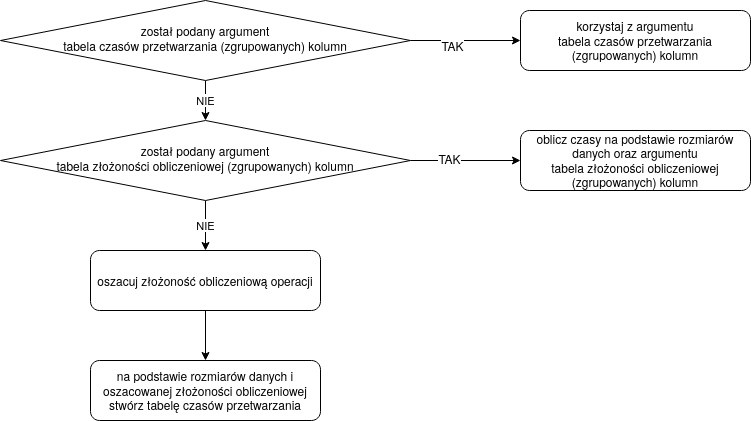
\includegraphics[width=.9\hsize]{fig/przydzielanie_czasow.png}
\caption{Schemat postępowania przy przydzielaniu czasu\label{diag:time-assign}}
\source{Opracowanie własne}
\end{figure}
\medskip

Poniżej opisane zostało zachowanie programu w zależności od podanych danych na temat czasu.

\subsubsection{Podano argument "tabela czasów przetwarzania (zgrupowanych) kolumn"}

W przypadku podania poprawnej macierzy czasów operacji ta część algorytmu nie jest wykonywana; zakładamy, że użytkownik podał prawidłowe wartości.
W szczególnym przypadku zadane mogą zostać jednakowe czasy wykonywania operacji.

\subsubsection{Podano argument "tabela złożoności obliczeniowej (zgrupowanych) kolumn"}

Ważnym aspektem tego argumentu, jest fakt, że w dziedzinie praktycznej podanie złożoności obliczeniowej nie może ograniczać się do podania samego asymptotycznego tempa wzrostu - $O(n)$; konieczne jest precyzyjniejsze oszacowanie funkcji wraz z czynnikiem dodanym (opóźnieniem, latencją).
\medskip

Jeżeli na wejściu do algorytmu znajduje się argument "tabela złożoności obliczeniowej (zgrupowanych) kolumn", jedyną operacją, która musi zostać wykonana jest podstawienie rozmiarów danych z poszczególnych komórek pod funkcje podane na wejściu.
\medskip

W szczególnym wypadku użytkownik może podać czasy niezależne od~rozmiaru wejścia - na przykład czasy jednostkowe.
\medskip

\subsubsection{Nie podano żadnego z argumentów odnoszących się do czasów przetwarzania}

Wiarygodne i uniwersalne oszacowanie czasów wykonywania różnych operacji nie jest możliwe.
Rozważono wprowadzenie systemu szacowania czasu na~podstawie analizy kilku (np. losowych, lub pierwszych) (zgrupowanych) wierszy - algorytm oszacuje złożoność operacji na danym procesorze, a następnie porówna rozmiar wejścia z czasem, w którym jest wykonywany.
Pakiet \emph{scipy.optimize} dostarcza funkcje do minimalizowania (lub~maksymalizowania) funkcji celu, z potencjalnymi ograniczeniami \cite{scipyoptimize}. Zawiera on~między innymi funkcjonalność \emph{curve\_fit} pozwalającą na znalezienie parametrów funkcji na~podstawie jej "szablonu" oraz porównania danych wejściowych i wyjściowych dla niej.
Funkcja działa wykorzystując metodą najmniejszych kwadratów korzystając z zadanego algorytmu, na przykład Levenberga-Marquardta \cite{lourakis2005brief}.

Wykorzystując ją mogłyby zostać dobrane parametry $a$, $b$, $c$ do funkcji
$$t = f(b * s^a + c)$$
Gdzie $t$ to czas wykonywania, a $s$ to rozmiar danych.\\
Niestety, mimo pokrycia części częstych przypadków, system byłby nieodporny na użycie jakichkolwiek funkcji, których czas wykonywania nie byłby pokryty tym modelem.
W związku z tym zrezygnowano z implementacji rzeczonego podsystemu i program zgłosi błąd w wypadku niepodania żadnego z argumentów odnoszących się do czasów przetwarzania.
\medskip


\section{Dobór algorytmu szeregowania}

Jeżeli użytkownik poda nazwę obsługiwanego przez program algorytm szeregowania, program wykorzysta swoją implementację tego algorytmu. W~przypadku niezaimplementowania wymaganego przez użytkownika algorytmu szeregowania program zgłosi błąd.
Należy dodać, że dodanie nowego algorytmu do systemu wymaga wyłącznie stworzenia klasy implementującej wymagane funkcje klasy bazowej wbudowanej w system i nie wymaga ingerencji w inne części kodu.
\medskip

Jeżeli algorytm szeregowania nie zostanie podany, to przy zadanym kryterium optymalizacyjnym program dobierze odpowiedni algorytm szeregowania służący do przygotowania optymalnego rozkładu.
\medskip

Dobór algorytmu polegał będzie na poruszaniu się po drzewie decyzji (bez~ingerencji użytkownika).
Wybór podjęty przez rozwiązanie funkcji zwracającej \emph{prawda/fałsz} na każdym poziomie prowadził będzie do kolejnej funkcji w~drzewie lub na poziomie liścia - do konkretnego algorytmu.


\section{Przygotowanie uszeregowania}

Po rozważeniu dwu metod możliwości rozdysponowania operacji pomiędzy procesory: z egzekutorem (koordynatorem) oraz w bez (w sposób nieskoordynowany) wybrana została metoda uwzględniająca egzekutora.
\medskip

Mimo większej prostoty mechanizmu, gdzie każdemu procesorowi zadana jest seria operacji do wykonania w określonych czasach, mechanizm z koordynatorem jest bardziej odporny na błędy i oferuje możliwość łatwiejszej rozbudowy.

Gdy przygotowane zostaną:

\begin{itemize}
    \item tabela wejściową z punkcie "Pobranie i preparacja danych",
    \item tabela czasów z punktu "Przydzielenie szacunkowych czasów wykonania poszczególnych operacji",
    \item graf konfliktu z wejścia,
    \item algorytm szeregowania z punktu "Dobór algorytmu szeregowania",
\end{itemize}

można przystąpić do konstrukcji uszeregowania.
\medskip

Konstrukcja uszeregowania polega na wykonaniu danego algorytmu szeregowania z danymi wejściowymi.
\medskip

Finalny rozkład zostanie zapisany w formie tabeli, której indeksy wierszy $t_t$ będą zawierały informacje o planowanym czasie rozpoczęcia wykonania operacji, kolumny $M_j$ przedstawiają procesory natomiast w komórce (kolejne małe litery alfabetu) znajduje indeks wiersza i kolumny zagregowanej tabeli wejściowej (lokalizacja komórki) w postaci dwójki [indeks wiersza, indeks kolumny].
\medskip

Przykładowy rozkład wynikowy został przedstawiony w tabeli \ref{tab:example-sched-out}.
\medskip

Należy zauważyć, że taki rozkład jest transponowanym klasycznym wykresem Gantta z dyskretnymi czasami rozpoczynania zadań.

\begin{table}[!tbh]
\begin{tabular}{|l|l|l|l|l|l|} \hline
Czas / proc & $M_1$     & $M_2$     & ...   & $M_{m-1}$ & $M_{m}$ \\ \hline
$t_1$       & $[a,b]$   & -         & ...   & $[c,d]$   & - \\ \hline
$t_2$       & -         & $[e,f]$   & ...   & -         & - \\ \hline
$t_3$       & $[e,f]$   & $[g,h]$   & ...   & -         & $[k,l]$\\ \hline
\end{tabular}
\caption{Przykładowe uszeregowanie wynikowe\label{tab:example-sched-out}}
\source{Opracowanie własne}
\end{table}


\section{Czuwanie nad prawidłowym wykonaniem rozkładu}

Egzekutor sekwencyjnie czytając wiersze rozkładu zajmował będzie się dysponowaniem operacji w momentach wynikających z indeksu wiersza na odpowiednie procesory.
\medskip

Idea działania egzekutora została przedstawiona na diagramie \ref{diag:executor}. Moment uchwycenia diagramu 
to czas 0, gdzie egzekutor odczytał pierwszy wiersz (z indeksem czasu 0) i rozdysponował operacje na komórce $[1,2]$ na~procesorze $M_1$ oraz komórki $[2,1]$ na procesorze $M_4$.
\medskip

\begin{figure}[!tbh]
\centering
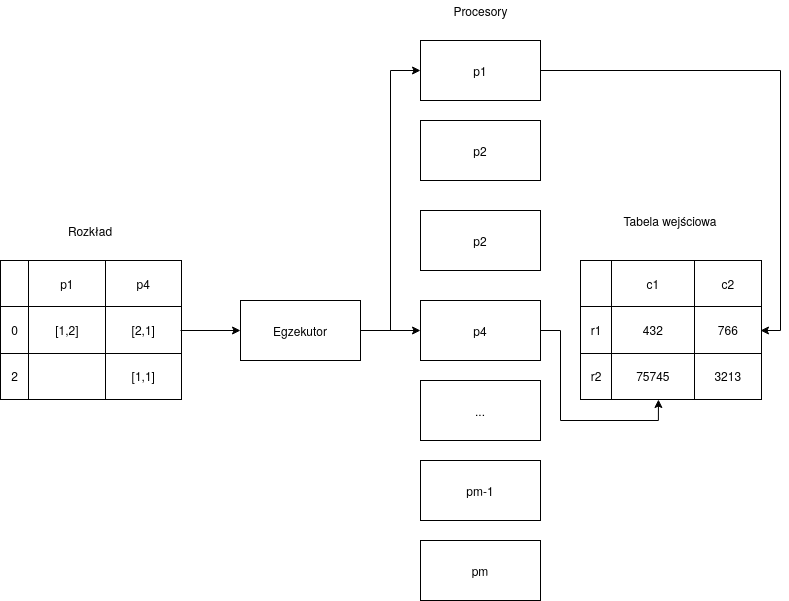
\includegraphics[width=.8\hsize]{fig/executor.png}
\caption{Schemat działania egzekutora\label{diag:executor}}
\source{Opracowanie własne}
\end{figure}
\medskip

Istnieje możliwość, w której oszacowanie czasu nie pokryło się z rzeczywistością. Sytuacja została szerzej opisana w rozdziale \ref{chap:extend}.\\

Na diagramach \ref{diag:sched_20j420} i \ref{diag:sched_100j4m} przedstawione zostały wykresy Gantta dla przykładowych problemów, z losowymi czasami operacji (zakres od~0~do~100~jednostek czasu). Na osi $x$ reprezentowany jest czas, oś $y$ - kolejne maszyny, natomiast zadania oznaczone są różnymi odcieniami szarości.

\begin{figure}[!tbh]
\centering
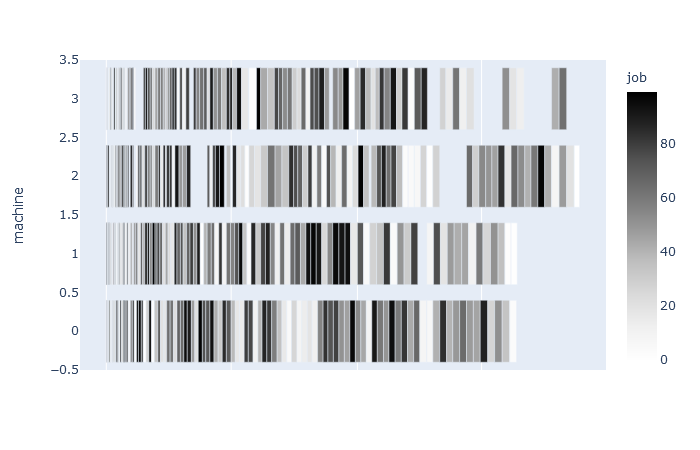
\includegraphics[width=.8\hsize]{fig/newplot_trim100j4m.png}
\caption{Przykładowe uszeregowanie dla 100 zadań i 4 maszyn\label{diag:sched_100j4m}}
\source{Opracowanie własne}
\end{figure}
\medskip

\begin{figure}[!tbh]
\centering
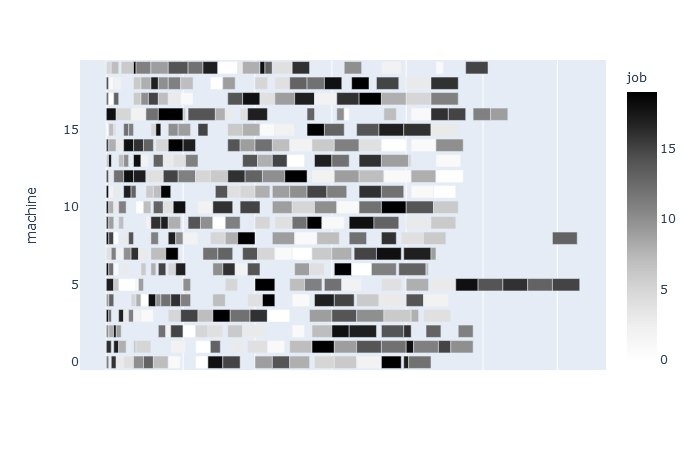
\includegraphics[width=.8\hsize]{fig/newplot_trim20j20m.png}
\caption{Przykładowe uszeregowanie dla 20 zadań i 20 maszyn\label{diag:sched_20j420}}
\source{Opracowanie własne}
\end{figure}
\medskip



\chapter{Algorytm wstawiania z wiązką szukającą}

W prototypie programu zaimplementowano heurystykę tworzenia uszeregowania zaproponowaną w~pracy \cite{grinshpoun2014partially} - wstawianie z wiązką szukającą (\emph{insertion with beam search}).
Jest ona adaptacją heurystyki zaproponowanej w~pracy \cite{brasel1993constructive}, która została w niej zastosowana do modelu szeregowania w~systemie otwartym.
Opiera się ona na wstawianiu kolejnych operacji (zgodnie z~ustaloną uprzednio kolejnością) do częściowego uszeregowania (\emph{partial schedule}), aż~do~momentu, gdy wszystkie operacje zostaną wstawione - co~jest~równoważne przygotowaniu pełnego uszeregowania. Częściowe uszeregowanie to~uszeregowanie posiadające właściwość, że jeżeli operacja $(i,j)$ poprzedza operację $(k,l)$, to moment ukończenia operacji $(i,j)$ jest wcześniejszy lub równy momentowi rozpoczęcia operacji $(k,l)$. Takie uszeregowanie jest~unikalne, zakładając częściową aktywność (\emph{semi-activeness}, operacje są wykonywane tak~szybko jak to jest możliwe, gdy ich kolejność jest znana) \cite{grinshpoun2014partially}.\\

Kolejność wstawiania operacji budowana jest następującym algorytmem:
\begin{enumerate}
    \item wyznacz $h = min\{n, m\}$ (mniejszą wartość z liczby kolumn i liczby wierszy w tabeli czasów przetwarzania),
    \item utwórz pustą listę operacji do wstawienia - $IO$,
    \item rozpoczynając w pierwszym wierszu, aż do $h-tego$ wiersza:
    \begin{enumerate}
        \item znajdź najdłuższy czas wykonywania spośród kolumn w tym wierszu,
        \item wstaw odpowiadającą jemu operację do $IO$,
        \item usuń kolumnę z tą komórką z tabeli,
        \item przejdź do następnego wiersza,
    \end{enumerate}
    \item kolejne operacje wstawiaj do $IO$ w porządku niemalejącym,
\end{enumerate}

Posiadając ustaloną kolejność wstawiania operacji można przystąpić do~dokładania ich do kolejnych częściowych uszeregowań. Przy każdym wstawieniu operacji $r_{ij}$ rozważamy następujące możliwości nadania jej rangi:
\begin{enumerate}
    \item $r_{ij} = 1$, co jest interpretowane jako: $i$ jest pierwszym zadaniem, które wykonuje maszyna $j$, oraz maszyna $j$ jest pierwszą (lub jedną z pierwszych) maszyn które pracują na zadaniu $i$,
    \item $r_{ij} = r_{kj} + 1$, gdzie $r_{kj}$ jest wartością w kolumnie $j$ częściowego uszeregowania, co interpretowane jest jako: operacja $(i, j)$ jest bezpośrednim następcą operacji $(k, j)$ na maszynie $j$,
    \item $r_{ij} = r_{il} + 1$, gdzie $r_{il}$ jest wartością w wierszu $i$ częściowego uszeregowania, a maszyny $j$ i $l$ są ze sobą w konflikcie, co jest interpretowane jako: operacja $(i, j)$ staje się bezpośrednim następcą operacji $(i, l)$ na~zadaniu $i$.
\end{enumerate}

Wstawienie operacji może spowodować, że częściowe uszeregowanie będzie niepoprawne. Dzieje się to, gdy tę samą rangę otrzymują operacja wstawiana oraz którakolwiek z operacji będących z nią w konflikcie:
\begin{enumerate}
    \item albo poprzez spowodowanie sytuacji, która przekłada się na wykonywanie dwóch lub więcej operacji na raz na jednej maszynie:
    $$\exists k \neq i, [r_{ij}=r_{kj}]$$
    \item albo wykonywanie dwóch lub więcej operacji połączonych krawędzią w~grafie konfliktu na raz:
    $$\exists l \neq j, [r_{ij}=r_{lj} \textrm{ oraz } (i,j) \textrm{ jest w konflikcie z } (i,l)]$$
\end{enumerate}
 
Powyższe sytuacje rozwiązywane są poprzez inkrementację wartości rangi dla operacji wcześniej wstawionych operacji. Należy zauważyć, że ten krok może spowodować wystąpienie nowych konfliktów, co wymaga powtarzania inkrementacji, aż do momentu, gdy częściowy rozkład będzie poprawny.\\

Po wstawieniu operacji do częściowego rozkładu następuje krok zastosowania wiązki szukającej.
Wiązka szukająca to zachłanna heurystyka przeszukiwania grafów wszerz, w której tylko ograniczona liczba najbardziej obiecujących ścieżek (dobranych według pewnego algorytmu) po każdym kroku zachowywana jest jako kandydaci - ich liczba nazywana jest szerokością wiązki.
W przypadku opisywanego programu stosowana jest metodyka wyboru najkrótszych najdłuższych ważonych ścieżek (wagami są czasy przetwarzania), przechodzących przez wstawianą operację.

Po wstawieniu ostatniej operacji z listy $IO$ wybrany zostaje jeden najlepszy kandydat i staje się on uszeregowaniem wynikowym w formie macierzy rang.
Uszeregowanie to jest następnie przekształcane w listę krotek zawierających czas rozpoczęcia operacji oraz maszynę i zadanie, które zostało zaszeregowane na ten moment. Taka lista konsumowania jest następnie przez~dyspozytor.
\medskip

Poniżej podany został przykład wstawiania operacji do częściowego uszeregowania.
Załóżmy, że dany jest problem z czterema maszynami\\
$\{M1, M2, M3, M4\}$ i czterema zadaniami $\{J1, J2, J3, J4\}$, oraz zadanymi czasami przetwarzania $PT$, jak w tabeli \ref{tab:example_pt}.
Niech ponadto wykonywanie tego samego zadania na maszynach $M1$ i $M4$ jednocześnie będzie niedozwolone.

\begin{table}[!tbh]
\begin{tabular}{|l|l|l|l|l|} \hline
     & $M1$ & $M2$ & $M3$ & $M4$ \\ \hline
$J1$ & 10 & 8 & 2 & 5 \\ \hline
$J2$ & 4 & 2 & 9 & 6 \\ \hline
$J3$ & 7 & 3 & 4 & 2 \\ \hline
$J4$ & 3 & 2 & 3 & 4 \\ \hline
\end{tabular}
\caption{Czasy przetwarzania $PT$ dla przykładu działania algorytmu wstawiania\label{tab:example_pt}}
\source{Opracowanie własne}
\end{table}\medskip

Algorytm zatrzymano w momencie, gdy do jednego z częściowych uszeregowań - kandydatów, wstawione zostały operacje widocznie na diagramie \ref{diag:state0}, a kolejną operacją do wstawienia jest $(J2, M4)$.\\
Na poprawnych uszeregowaniach w poniższych diagramach zaznaczono częściowy graf sekwencji.

\begin{figure}[!tbh]
\centering
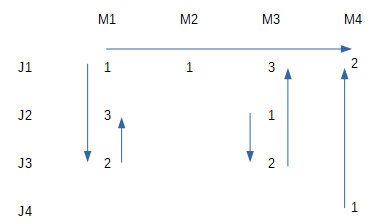
\includegraphics[width=.7\hsize]{fig/0.png}
\caption{Częściowe uszeregowanie przed wstawieniem operacji $(J2, M4)$\label{diag:state0}}
\source{Opracowanie własne}
\end{figure}\medskip

\begin{figure}[!tbh]
\centering
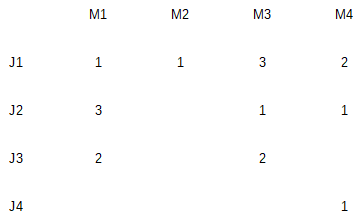
\includegraphics[width=.7\hsize]{fig/1_0.png}
\caption{Wariant 1. nadania rangi: nadanie rangi $1$ - uszeregowanie jest~niepoprawne przez tę samą rangę dla $(J2, M4)$ i $(J4, M4)$\label{diag:state1_0}}
\source{Opracowanie własne}
\end{figure}\medskip

\begin{figure}[!tbh]
\centering
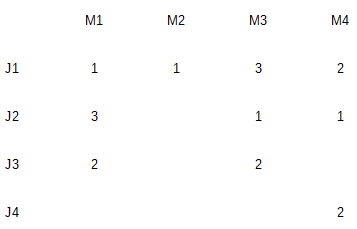
\includegraphics[width=.7\hsize]{fig/1_1.png}
\caption{Inkrementacja rangi $(J4, M4)$ - uszeregowanie jest niepoprawne przez tę samą rangę dla $(J4, M4)$ i $(J1, M4)$\label{diag:state1_1}}
\source{Opracowanie własne}
\end{figure}\medskip

\begin{figure}[!tbh]
\centering
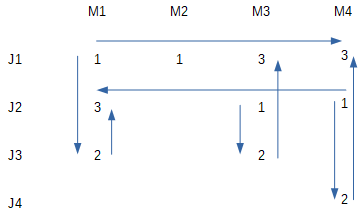
\includegraphics[width=.7\hsize]{fig/1.png}
\caption{Inkrementacja rangi $(J1, M4)$ - uszeregowanie jest poprawne, a~najdłuższa ścieżka przechodząca przez wstawianą operację ma długość $6 + 4 + 5 = 15$, lub $10 + 5 = 15$\label{diag:state1}}
\source{Opracowanie własne}
\end{figure}\medskip
 
\begin{figure}[!tbh]
\centering
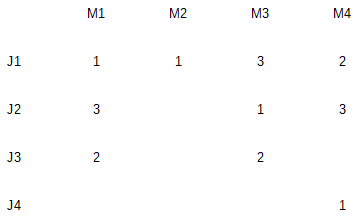
\includegraphics[width=.7\hsize]{fig/3_1.png}
\caption{Wariant 2. nadania rangi: nadanie rangi o $1$ większej niż $(J1, M4)$ - uszeregowanie jest niepoprawne przez tę samą rangę dla $(J2, M4)$ i $(J2, M1)$\label{diag:state3_1}}
\source{Opracowanie własne}
\end{figure}\medskip

\begin{figure}[!tbh]
\centering
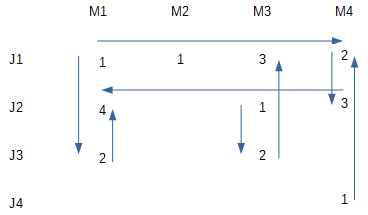
\includegraphics[width=.7\hsize]{fig/2.png}
\caption{Inkrementacja rangi $(J2, M1)$ - uszeregowanie jest poprawne, a~najdłuższa ścieżka przechodząca przez wstawianą operację ma długość $10 + 5 + 6 + 4 = 25$\label{diag:state2}}
\source{Opracowanie własne}
\end{figure}\medskip

\begin{figure}[!tbh]
\centering
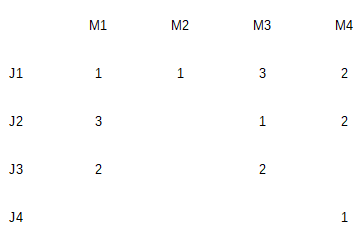
\includegraphics[width=.7\hsize]{fig/3_0.png}
\caption{Wariant 2. nadania rangi: nadanie rangi o $1$ większej niż $(J4, M4)$ - uszeregowanie jest niepoprawne przez tę samą rangę dla $(J2, M4)$ i $(J1, M4)$\label{diag:state3_0}}
\source{Opracowanie własne}
\end{figure}\medskip

\begin{figure}[!tbh]
\centering
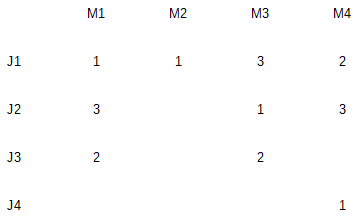
\includegraphics[width=.7\hsize]{fig/3_1.png}
\caption{Inkrementacja rangi $(J1, M4)$ - uszeregowanie jest niepoprawne przez tę samą rangę dla $(J2, M1)$ i $(J2, M4)$\label{diag:state3_1}}
\source{Opracowanie własne}
\end{figure}\medskip

\begin{figure}[!tbh]
\centering
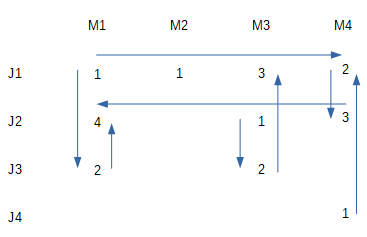
\includegraphics[width=.7\hsize]{fig/3.png}
\caption{Inkrementacja rangi $(J2, M1)$ - uszeregowanie jest poprawne, a~najdłuższa ścieżka przechodząca przez wstawianą operację ma długość $10 + 5 + 6 + 4 = 25$\label{diag:state3}}
\source{Opracowanie własne}
\end{figure}\medskip

\begin{figure}[!tbh]
\centering
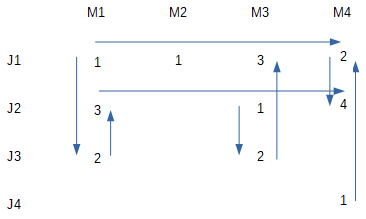
\includegraphics[width=.7\hsize]{fig/4.png}
\caption{Wariant 3. nadania rangi: nadanie rangi o $1$ większej niż~$(J2, M1)$ - uszeregowanie jest poprawne, a najdłuższa ścieżka przechodząca przez~wstawianą operację ma długość $10 + 7 + 4 + 6 = 27$\label{diag:state4}}
\source{Opracowanie własne}
\end{figure}\medskip

Analogiczne kroki wykonywane są na każdym z częściowych uszeregowań - kandydatów.
Po zebraniu długości najdłuższych ścieżek przechodzących przez wstawianą operację w każdym z nich, na podstawie tych długości wybrane zostaje nowe grono najbardziej obiecujących częściowych uszeregowań - kandydatów, ograniczone szerokością wiązki.
Wstawianie kolejnej operacji w kolejności rozpoczyna ten cykl na nowo.



\chapter{Analiza sprawności dyspozytora}

W celu analizy sprawności dyspozytora przeprowadzono serię testów.
Testy różniły się między sobą:
\begin{enumerate}
    \item liczbą kolumn,
    \item liczbą wierszy,
    \item czasem wykonywania poszczególnych operacji,
    \item grafem konfliktu.
\end{enumerate}

Wyniki testów dla algorytmu wstawianie z wiązką szukającą (\emph{insertion with beam search}) określają potencjalne jego zastosowania. Są to albo zbiory danych, gdzie liczby wierszy i kolumn po zgrupowaniu są bardzo małe (na~przykład kilkadziesiąt wierszy i kilka kolumn), albo operacje, których naiwne zrównoleglanie trwa bardzo długo (wiele godzin). Naturalnie istnieje wiele takich przypadków, gdzie pożądanym jest sprowadzenie poprzez grupowanie dużych liczb wierszy do niewielu grup, lub operacji, których czas wykonania jest liczony w dniach. Na wykresach \ref{diag:relplot_128j} i \ref{diag:relplot_16m} znajdują się wykresy czasów przygotowania uszeregowań w zależności od, odpowiednio, liczby maszyn i~liczby zadań. Widać na nich złożoność obliczeniową - $O(n)=n^4$ względem liczby zadań (podobnie jak w oryginalnej pracy \cite{brasel1993constructive}) i $O(n)=n$ względem liczby maszyn (dzięki zastosowaniu uproszczonego sprawdzania konfliktów).

\begin{figure}[!tbh]
\centering
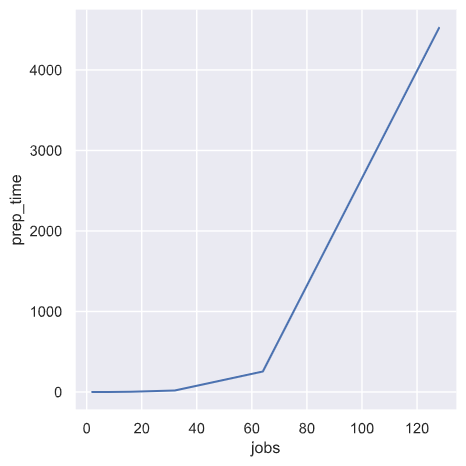
\includegraphics[width=.8\hsize]{fig/relplot_128j.png}
\caption{Porównanie czasu przygotowania uszeregowania dla 16 maszyn w~zależności od liczby zadań\label{diag:relplot_128j}}
\source{Opracowanie własne}
\end{figure}\medskip

\begin{figure}[!tbh]
\centering
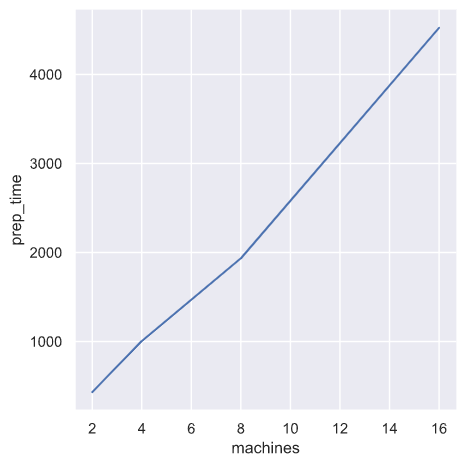
\includegraphics[width=.8\hsize]{fig/relplot_16m.png}
\caption{Porównanie czasu przygotowania uszeregowania dla 128 zadań w~zależności od liczby maszyn\label{diag:relplot_16m}}
\source{Opracowanie własne}
\end{figure}\medskip



\chapter{Analiza sprawności algorytmów dla podproblemu}

W celu analizy sprawności algorytmu wstawiania z wiązką szukającą (\emph{insertion with beam search}) porównano sumę czasów działania dyspozytora oraz~wykonywania sekwencyjnego wszystkich operacji.

Stosunki czasów $C_{max}$ (heurystyka do naiwnego) w zależności od liczby zadanych komórek znajdują się na wykresie diagnostycznym \ref{diag:time_ratio_2}. Wartości, które można odczytać z wykresu wskazują na bardzo duże oszczędności czasu, w szczególności wraz ze wzrostem liczby wykonywanych zadań.

\begin{figure}[!tbh]
\centering
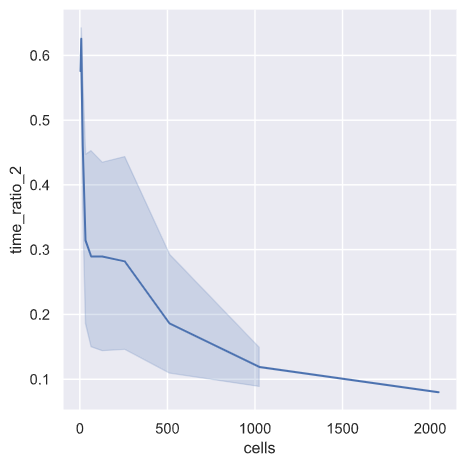
\includegraphics[width=.7\hsize]{fig/time_ratio_2.png}
\caption{Stosunki czasu wykonywania operacji zgodnie z heurystyką do~naiwnego wykonania \label{diag:time_ratio_2}}
\source{Opracowanie własne}
\end{figure}\medskip



\chapter{Potencjalne kierunki rozwoju pracy} \label{chap:extend}

Praca otwiera kilka tematów, o które może być rozszerzona oraz kilka potencjalnych tematów nowych prac.
\medskip

W celu pełnego wprowadzenia systemu do użycia, należy rozwiązać problem potencjalnych różnic pomiędzy założonym czasem operacji a czasem rzeczywistym. System obecnie stosuje margines bezpieczeństwa (niewielką wartość dodaną do szacowanego czasu operacji).
W pełni rozwinięty system powinien mieć tolerancję na takie błędy i wprowadzać korekty do rozkładu w trakcie jego wykonywania.
\medskip

Jako całkiem nowy temat, wartościowym byłoby poddanie analizie prawdopodobnie częściej spotykanego przypadku pominięcia grafu konfliktu, czyli~zaimplementowania systemu dla modelu wieloprocesorowego systemu otwartego (\emph{Multiprocessor Open Shop Schedule}).
\medskip

Kolejnym tematem, który został zauważony w trakcie analizy zagadnienia są szczególne (a zarazem najczęstsze) przypadki \emph{PCOSS}, gdy graf konfliktu sprowadza się do grafu konfliktu wyłącznie dla kolumn, tj. z pominięciem krawędzi "pionowych" (między wierszami). Daje to potencjał do znalezienia i zastosowania bardziej optymalnych algorytmów.
\medskip

Zaproponowany system można zaimplementować jako tzw. \emph{scheduler}, na~przykład w module \emph{Dask} \cite{dask} języka \emph{Python}, który jest powszechnie stosowany przy zrównolegnianiu operacji na \emph{DataFrame-ach}.



\summary

W pracy zaproponowano model systemu pozwalającego na redukcję czasu wykonywania serii operacji na danych tabelarycznych. System taki, prawdopodobnie z uwagi na specyficzną grupę odbiorców, nie został zaimplementowany w żadnym ze znanych modułów dostępnych w powszechnych językach programowania.
\medskip

Wybór problemu szeregowania zadań częściowo zależnych w systemie otwartym został podyktowany jego największą generalizacją spośród problemów typu powszechnych systemów szeregowania na maszynach dedykowanych. Jego ograniczanie do innych problemów nie powinno przynosić dużych wyzwań.
\medskip

Praca otwiera drogę do jej rozszerzenia, implementacji w komercyjnych produktach oraz optymalizacji.
\medskip

Najbardziej aktualną wersję kodu źródłowego systemu oraz wybudowany program serwera można znaleźć pod adresem:\\ \url{https://github.com/ksazon/pcoss}\\
Na stronie znajduje się plik README.md, w którym znajdują się informacje na temat tego, w jaki sposób uruchomić program.

% % załączniki (opcjonalnie):
% \appendix
% \chapter{Tytuł załącznika jeden}

% Treść załącznika jeden.

% \chapter{Tytuł załącznika dwa}

% Treść załącznika dwa.

% literatura (obowiązkowo):
% \bibliographystyle{unsrt}
% \bibliography{xml}


% \addbibresource{xml.bib}
\printbibliography[nottype=online,title={Bibliografia}]
\printbibliography[type=online,title={Źródła internetowe}]
% spis tabel (jeżeli jest potrzebny):
\listoftables

% spis rysunków (jeżeli jest potrzebny):
\listoffigures

\oswiadczenie

\end{document}
